%============================================================ 4. 제안 방법 (압축판)
%  원판(sections_real/04_method.tex)에서 구현 세부 수식을 산문으로 내리고, 결과에 쓰이지
%  않은 반사실 크레딧 변형을 덜어냈다. 남긴 식은 방법의 정체성을 정하는 것들이다.
\section{제안 방법}
\label{sec:method}

\subsection{2계층 비동기 구조}
\label{sec:arch}

전략 계층은 어느 방어정이 어느 적 무리를 맡는가를, 기동 계층은 어느 위치에 그물을 놓는가를
정한다(Fig.~\ref{fig:architecture}). 언어모델 호출에는 지연이 있으므로(\ref{sec:res_latency}절),
기동 계층이 그 응답을 기다리느라 늦어지지 않도록 전략 계층만 비동기로 분리한다. 기동 계층은
배정 응답을 기다리는 동안 직전 배정으로 결정을 계속하고, 응답이 도착하면 다음 결정부터 새
배정을 반영한다.

\subsection{적 무리 군집화}
\label{sec:cluster}
\begin{figure}[!htbp]
\centering
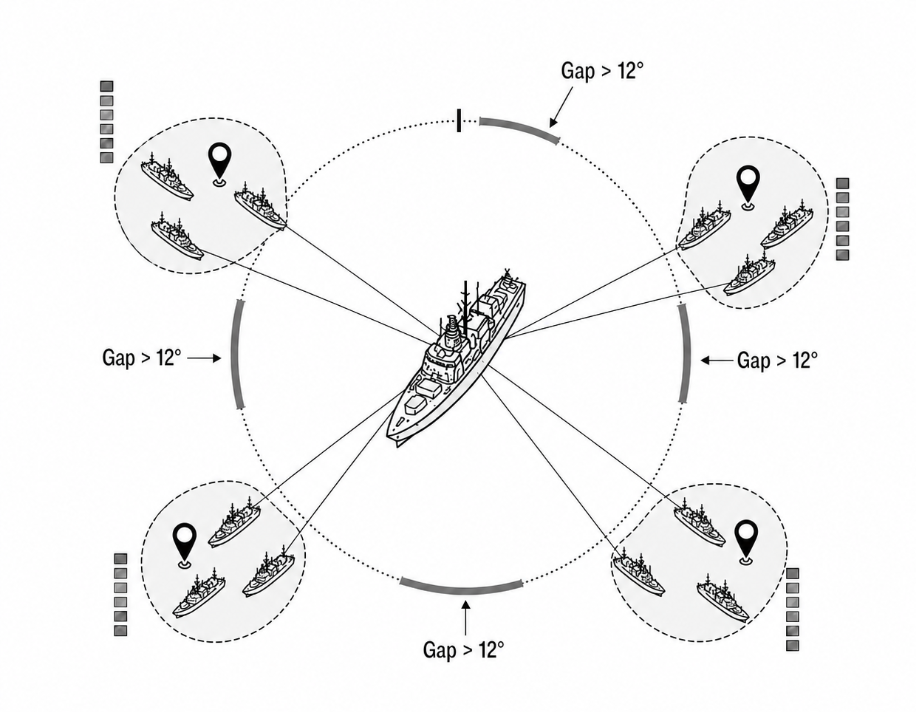
\includegraphics[width=0.8\columnwidth]{fig5.png}
\caption{방위각 정렬, 군집화, 군집 배정}
\label{fig:clustering}
\end{figure}

두 계층 모두 개별 적 USV가 아니라 무리를 단위로 다루므로, 매 결정마다 생존 적 USV $n$척을
모선에서 본 방위 $\vartheta_m$ 순으로 정렬해 최대 $C$ 개의 무리로 묶는다(Fig.~\ref{fig:clustering}).
방위 구간을 고정해 나누면 한 무리가 경계에 걸려 쪼개질 수 있으므로, 원을 따라 이웃한 방위 사이의
간격 $g_{(q)}$ 가운데 크게 벌어진 곳을 무리의 경계로 삼아 무리 수를 적의 분포에 따라 정한다.
임계 $\delta_{\mathrm{gap}}$ 을
넘는 간격의 개수가 활성 무리 수 $\hat{C}$ 이며, 이를 $1$ 이상 $\min(C, n)$ 이하로 제한한다.
\begin{equation}
\hat{C} = \mathrm{clip}\!\Big(\big|\{\, q : g_{(q)} > \delta_{\mathrm{gap}} \,\}\big|,\; 1,\; \min(C, n)\Big)
\label{eq:ncluster}
\end{equation}
가장 큰 간격 $\hat{C}$ 개를 경계로 삼아 방위 순으로 무리를 나누고, 각
무리를 척수 $n_j$, 중심 $\mathbf{c}_j$, 각도 퍼짐 $\Delta\vartheta_j$, 모선 방향 접근 속도
$v^{\mathrm{app}}_j$ 의 네 양으로 요약한다. 이 규칙에 따르면 집중은 무리 하나, 양동은 셋으로 요약되며, 파상은 대개 차례로 밀려오는 무리마다
하나씩으로 요약된다.
% ★ Fig.6(fig:observation) 은 2단 figure* 라 선언된 쪽에 놓일 수 없어 여기(§4.2 끝)에서
%   선언해야 §4.4.1 이 시작하는 쪽 상단에 앉는다.
\begin{figure*}[!tp]
\centering
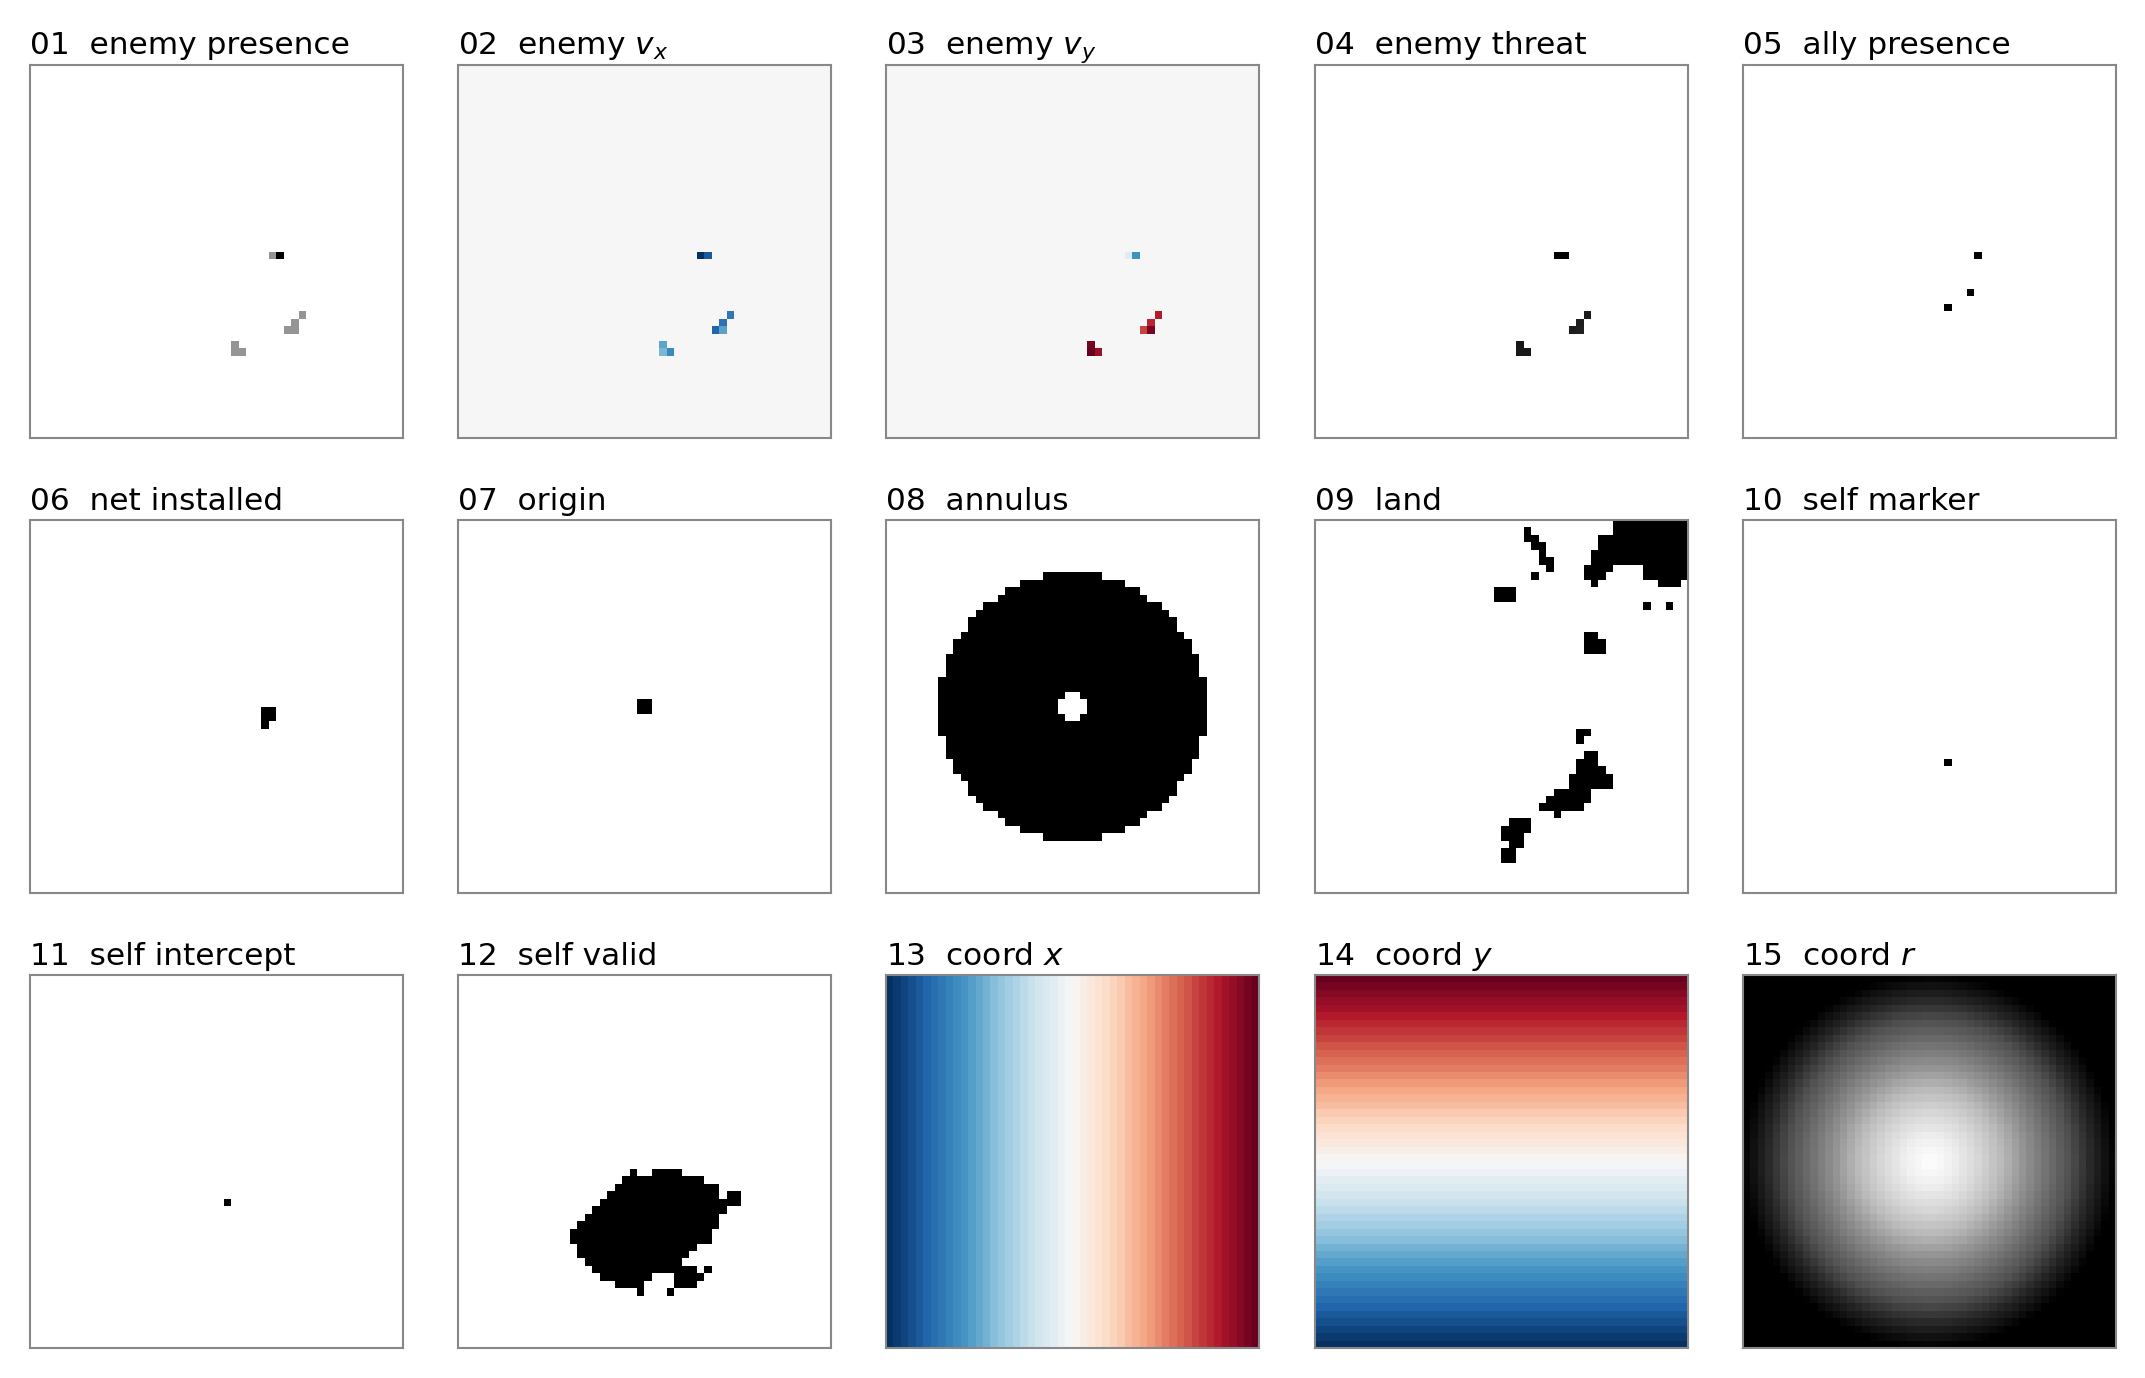
\includegraphics[width=0.62\textwidth]{fig6.png}
\caption{래스터화된 15채널 관측의 예(파상, 통영 매물도 북측)}
\label{fig:observation}
\end{figure*}

\subsection{기하 휴리스틱 기준 방법}
\label{sec:heuristic}

무리 요약 위에서 같은 문제를 기하 규칙만으로 푸는 기준 방법으로, \ref{sec:results}절의 비교
기준이자 \ref{sec:bc}절의 행동 복제 목표다. 무리 $j$ 의 위협도 $\tau_j$ 는 척수 $n_j$ 에 모선
근접도를 곱한 양이고, 요격점 $\mathbf{I}_j$ 는 무리 중심에서 모선을 향해 선분의 $\lambda_{\mathrm{I}}$
비율만큼 옮긴 점이다.
\begin{equation}
\begin{aligned}
\tau_j &= n_j \cdot \mathrm{clip}\!\left(1 - \frac{\lVert \mathbf{c}_j - \mathbf{m}\rVert}{R_w},
         \, 0.05,\, 1\right),\\
\mathbf{I}_j &= \mathbf{c}_j + \lambda_{\mathrm{I}}\,(\mathbf{m} - \mathbf{c}_j), \qquad \lambda_{\mathrm{I}} = 0.55
\end{aligned}
\label{eq:threat}
\end{equation}
방어정이 적보다 느리므로 요격점은 모선 쪽으로 치우쳐 둔다.

위협 상위 $P$ 개 무리에 대해 Greedy 1:1 배정을 한다. 비용은 방어정 위치 $\mathbf{a}_p$ 에서
요격점까지의 거리 $d_{pj}$ 에서, 직전 결정의 담당 $j_p^{\text{prev}}$ 를 유지하는 쌍에만
보너스 $\beta$ 를 감한 값으로, 거리 차이가 크게 벌어지기 전에는 직전 배정이 유지된다.
\begin{equation}
\tilde{d}_{pj} = \begin{cases}
  d_{pj} - \beta, & \text{if } j = j_p^{\text{prev}},\\
  d_{pj},          & \text{otherwise}.
\end{cases}
\label{eq:sticky}
\end{equation}
활성 무리가 $P$ 보다 적으면 남는 방어정은 한 척당 맡는 적이 가장 많은 무리에 추가로 배정되어
기존 요격점보다 모선에 가까운 곳에서 그 무리를 한 번 더 막는다. 그물은 요격점을 가운데 두고 접근
방향에 수직으로 길이 $L_{\mathrm{net}}$ 만큼 펼치므로 경유점은 양 끝 $K = 2$ 개이며, 학습 정책과
같은 격자 위에서 갈 수 있는 가장 가까운 칸으로 맞춘다. 따라서 휴리스틱과 학습 정책은 같은
행동공간을 쓰며, 다른 것은 결정 규칙뿐이다.

\subsection{점수맵 기반 기동 정책}
\label{sec:policy}

\subsubsection{다채널 격자 관측}
\label{sec:obs}

기동 계층의 입력은 좌표 목록이 아니라, 모선을 중앙에 두고 사방으로 $E$ 까지의 전장을
$n_{\mathrm{g}} \times n_{\mathrm{g}}$ 격자로 나눈 다채널 지도이다. 15개 채널은 모든 방어정이
공유하는 전역 9채널, 방어정마다 다른 3채널, 좌표 3채널로 구성된다(Fig.~\ref{fig:observation}).
한 칸의 크기는 $\ell = 2E/n_{\mathrm{g}}$ 이며, 각 선박의 위치를 해당 칸에 표시하고 한 칸에 여러
척이 있으면 합산한다. 방어정 $p$ 의 자체 상태 $\mathbf{o}_p \in \mathbb{R}^{8}$ 는 지도와 별도로
입력한다. 모든 입력은 $\ell$ 단위의 무차원 값이고, 지도는 선박이 몇 척이든 어떤 순서로 나열되든
같은 크기로 만들어지므로, 해역 크기나 선박 수가 바뀌어도 입출력의 형태가 같다.

\subsubsection{FiLM 조건화 U-Net과 점수맵}

\begin{figure*}[!tbp]
\centering
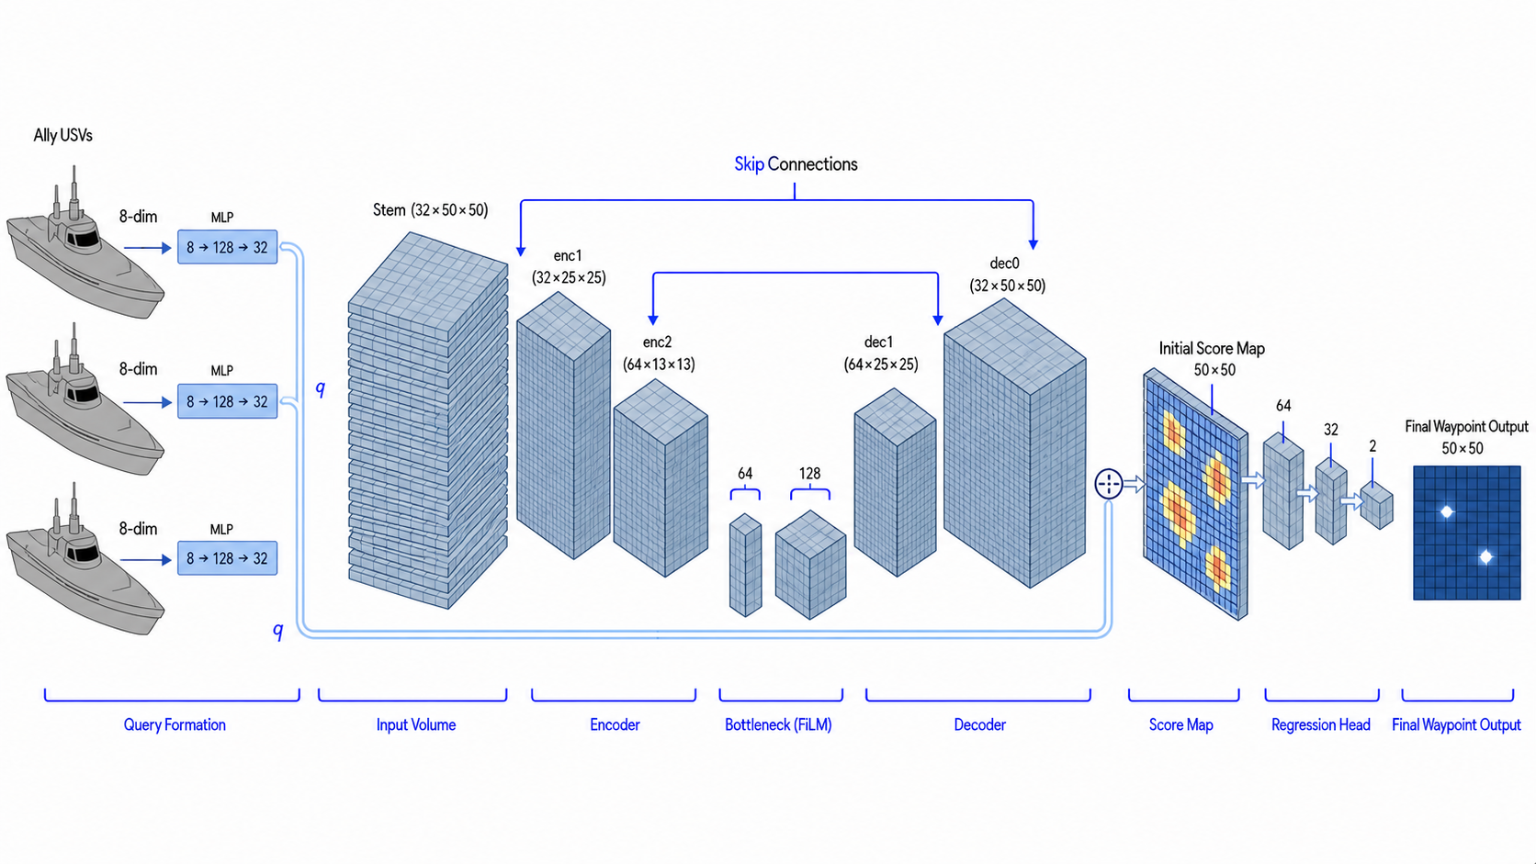
\includegraphics[width=0.66\textwidth]{fig8.png}
\caption{점수맵 정책의 구조: 질의·특징맵 내적과 칸 안 오프셋}
\label{fig:policy}
\end{figure*}

관측은 U-Net 구조~\citep{ronneberger2015unet}를 지나 입력과 같은 해상도의 특징 지도로
변환된다(Fig.~\ref{fig:policy}). 전역 평균 풀링으로 압축한 전황 벡터는
FiLM~\citep{perez2018film} 변조로 특징에 실려, 국소 합성곱이 옮기지 못하는 전황을 모든 위치에
전달한다.

각 방어정 $p$ 는 자신의 상태 벡터 $\mathbf{o}_p$ 로부터 MLP 로 질의 $\mathbf{q}_p$ 를 만들고,
아핀 사영 $\mathbf{W}_q$, $\mathbf{b}_q$ 를 거쳐 픽셀 $i$ 의 특징 $\mathbf{f}_i$ 와 내적하여
점수 $s_{p,i}$ 를 얻는다.
\begin{equation}
s_{p,i} = \frac{\langle \mathbf{W}_q \mathbf{q}_p + \mathbf{b}_q,\, \mathbf{f}_i \rangle}{\sqrt{d}}, \qquad d = 32
\label{eq:score}
\end{equation}
어텐션~\citep{vaswani2017attention}과 같은 형식의 점수로 격자 위의 원소를 지목하는 포인터
구조다~\citep{vinyals2015pointer}. 가중치는 모든 방어정이 공유하므로 모델 크기는 방어정 수에 불변이다.

\subsubsection{유효 마스크와 픽셀 지목}
\label{sec:validmask}

점수맵 전체가 후보가 되는 것은 아니다. 육지 픽셀 집합을 $\mathcal{L}_{\mathrm{land}}$, 모선에서
본 요격점 방위와 픽셀 방위의 차이를 $[0^\circ, 180^\circ]$ 로 접은 값을
$|\vartheta_i - \vartheta_p|_{\circ}$ 라 하면, 방어정 $p$ 의 유효 픽셀 집합 $\mathcal{V}_p$ 는
환상 요격 구역($r_{\min} = 1.6\,\ell$, $r_{\max} = 18\,\ell$), 육지 밖, 요격점 반경
($r_{\mathrm{g}} = 12\,\ell$), 무리 방위($\vartheta_{\mathrm{g}} = 60^\circ$)라는 네 조건의 교집합이다.
\begin{equation}
\begin{aligned}
\mathcal{V}_p = \big\{\, i :\; & r_{\min} \le \lVert \mathbf{x}_i - \mathbf{m} \rVert \le r_{\max},\;
  i \notin \mathcal{L}_{\mathrm{land}},\\
  & \lVert \mathbf{x}_i - \mathbf{I}_p \rVert \le r_{\mathrm{g}},\;
  |\vartheta_i - \vartheta_p|_{\circ} \le \vartheta_{\mathrm{g}} \,\big\}
\end{aligned}
\label{eq:validset}
\end{equation}
마스크는 로짓 단계에서 적용한다. 유효 집합 밖의 점수를 $-\infty$ 로 바꾼 마스크 점수
$\tilde{s}_{p,i}$ 를 소프트맥스에 넣어 픽셀 선택 확률을 얻는다.
\begin{equationsmall}
\tilde{s}_{p,i} = \begin{cases} s_{p,i}, & i \in \mathcal{V}_p \\ -\infty, & i \notin \mathcal{V}_p, \end{cases}
\quad
\pi_\theta(i \mid \mathbf{s}, p) = \frac{e^{\tilde{s}_{p,i}}}{\sum_{j \in \mathcal{V}_p} e^{\tilde{s}_{p,j}}}
\label{eq:masked_softmax}
\end{equationsmall}
제약이 손실 항이 아니라 행동 분포에 직접 부과되므로 위반은 애초에 표현 불가능하며, 학습된
체크포인트에서 격자 대부분은 갈 수 없는 자리로 남는다(Fig.~\ref{fig:validmask}).


\begin{figure*}[tbp]
\centering
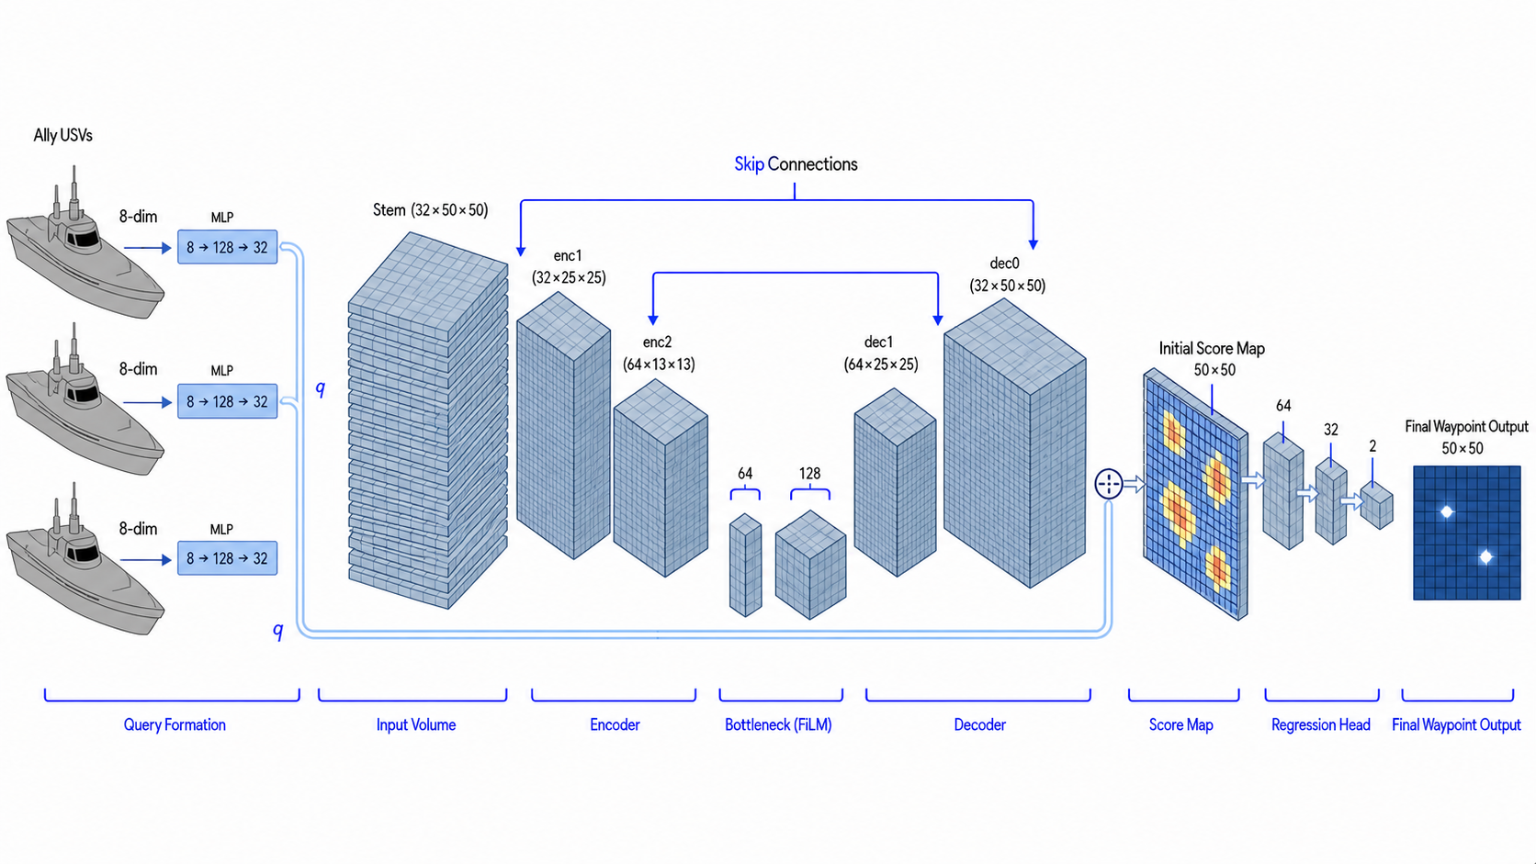
\includegraphics[width=\textwidth]{fig9.png}
\caption{유효 마스크와 픽셀 지목(학습된 체크포인트의 실제 출력)}
\label{fig:validmask}
\end{figure*}

각 방어정은 유효 영역 안에서 픽셀 $K$ 개를 순차적으로 고르며, 먼저 고른 픽셀의 특징을 질의에
더해 두 번째를 고르므로 두 점이 서로를 알고 뽑힌다. 칸 안 위치는 가우시안 오프셋으로 정하고,
두 점을 잇는 선분이 그물 경로가 된다.

\subsection{가치망 없는 다중 에이전트 그룹 상대 최적화}
\label{sec:training}



\subsubsection{그룹 상대 이득}

학습은 가치함수를 따로 두지 않는 그룹 상대 정책 최적화~\citep{shao2024deepseekmath}를 다중
방어정 상황에 맞게 변형하여 수행한다. 매 결정 시점에서 정책으로부터
$G$개의 결합 행동 후보를 표집하되, 후보 가운데 하나($k=0$)는 휴리스틱(\ref{sec:heuristic}절)이
내는 행동으로 고정하여 기준선으로 삼는다. 각 후보를 시뮬레이터에서 공통 구간
$H = 180\,\mathrm{step}$ 만큼 실제로 진행시켜 창 보상 $R_k$ 를 얻은 뒤(\ref{sec:reward}절),
휴리스틱 후보의 보상 $R_0$ 를 기준으로 상대 비교하여 이득 $A_k$ 를 산정한다. 그룹 표준편차로 나누되 $\epsilon$ 을 더해 0 나눗셈을 막는다.
\begin{equation}
A_k = \frac{R_k - R_0}{\mathrm{std}(\{R_j\}_{j=0}^{G-1}) + \epsilon}
\label{eq:adv}
\end{equation}
휴리스틱을 넘어서는 후보만 양의 이득을 받으며, 실제 결과를 직접 비교하므로 가치망과 그 추정
편향이 없다. 한 갱신은 $N$개의 병렬 전장(월드)에서 수행되고, 후보 보상이 모두 같은 월드는 유효
월드 마스크 $w_n$ 으로 제외한다. 월드 $n$ 의 상태를
$\mathbf{s}_n$, 후보 $k$ 의 이득을 $A_{n,k}$, 그 후보에서 방어정 $p$ 의 행동을
$a^{(k)}_{n,p}$ 라 하면 정책경사 손실은 다음과 같다.
\begin{equationfn}
\mathcal{L}_{\mathrm{PG}}(\theta) = -\frac{\sum_{n} w_n \sum_{k=0}^{G-1} A_{n,k} \sum_{p=1}^{P} \log \pi_\theta\big(a^{(k)}_{n,p} \mid \mathbf{s}_n\big)}{G \sum_n w_n}
\label{eq:lpg}
\end{equationfn}
여기에 엔트로피 정칙화를 더한 총손실을 최소화하며, 기울기 노름을 클립한 뒤 갱신한다.

\label{sec:bc}
\label{sec:schedule}
그룹 상대 이득은 후보들이 갈릴 때만 신호를 주므로, 학습에 앞서 휴리스틱 픽셀 중심의 폭 좁은
가우시안을 목표로 한 행동 복제로 정책을 부팅한다. 옵티마이저는 Adam 이며, 학습률은 $10^{-4}$ 에서 그 $5\,\%$ 까지
단일 주기 코사인 어닐링으로, 엔트로피 계수는 $0.01$ 에서 그
$10\,\%$ 까지 선형으로, 총 800 업데이트의 같은 예산 축 위에서 함께 줄인다. 병렬 전장은 24개, 그룹 크기는 휴리스틱 후보를 포함해 $G = 8$, 행동 복제는
300 갱신이다.

\begin{figure*}[tbp]
\centering
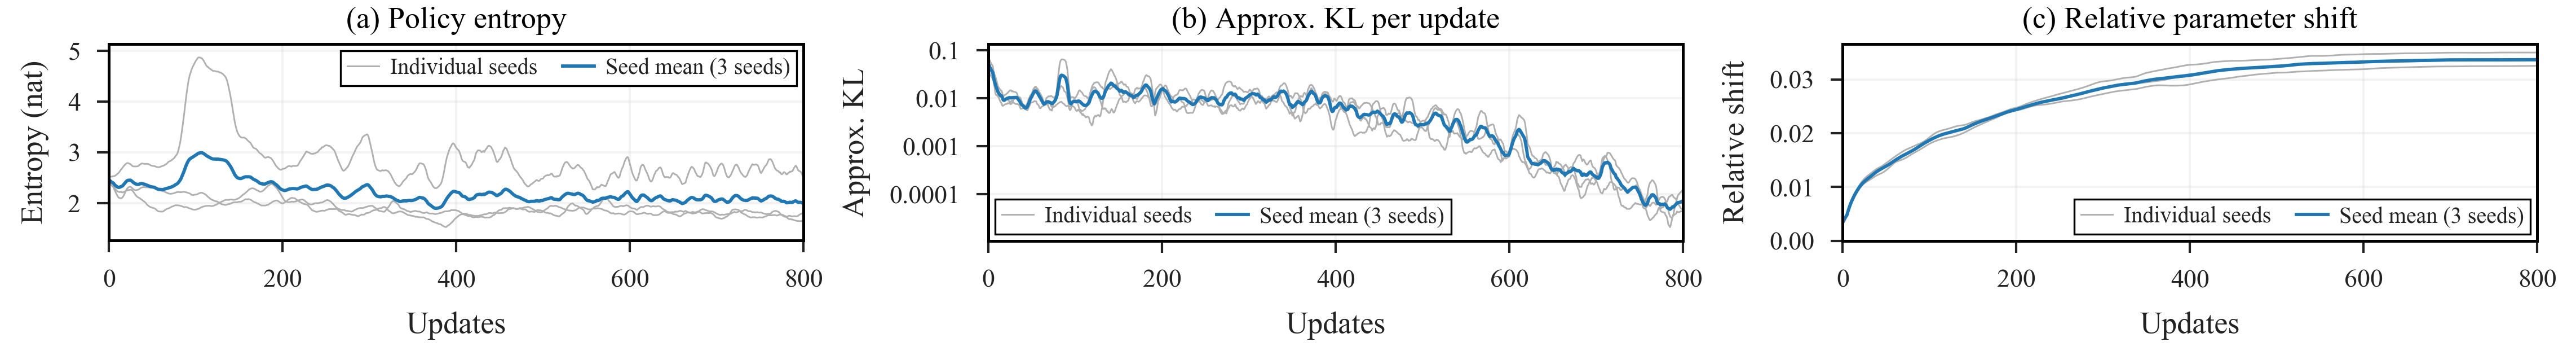
\includegraphics[width=\textwidth]{fig12_h3.png}
\caption{학습 경과(회색 시드별, 파란 실선 시드 평균): (a) 정책 엔트로피, (b) 근사 KL 발산,
         (c) 행동 복제 초기점 대비 파라미터 이동}
\label{fig:convergence}
\end{figure*}

같은 설정을 시드 3개로 반복해 학습 경과를 기록하였다(Fig.~\ref{fig:convergence}). 갱신 전후
정책 사이의 근사 KL은 처음 100 업데이트 평균 $1.4\times10^{-2}$ 에서 마지막 100 업데이트
$1.5\times10^{-4}$ 로 두 자릿수 줄고, 파라미터 이동은 후반에 포화하며, 정책 엔트로피는
$2.42$ 에서 $2.06$\,nat 로 내려가 400 업데이트 이후 평탄하다. 학습이 끝난 800 업데이트에서
세 시드의 greedy 포획률은 모두 휴리스틱 기준선 $0.749$ 를 넘는다.

\subsubsection{보상 설계}
\label{sec:reward}

한 후보의 창 보상은 결정 시점부터 $H$\,step 동안의 팀 공유 보상으로, 이벤트 항 $R_\mathrm{event}$,
창의 시작·끝 상태에서 잰 퍼텐셜 $\Phi$ 의 할인($\gamma = 0.99$) 차분, 조밀 항 $R_\mathrm{dense}$ 로
구성된다.
\begin{equation}
R = R_\mathrm{event} + \big[\gamma\,\Phi(\mathbf{s}_{t+H}) - \Phi(\mathbf{s}_t)\big] + R_\mathrm{dense}
\label{eq:reward}
\end{equation}
이벤트 항은 포획($+13.5$)·돌파($-8$)·충돌($-30$)·그물 접촉($-13$) 건수의 가중합이고, 퍼텐셜은
생존 적선의 모선 근접도 합의 음수라 할인 차분 형태로 최적 정책을 보존한다~\citep{ng1999shaping}.
조밀 항은 이동거리·그물 소모·선회량·목표점 변경·근접도를 벌하고 그물의 접근로 차단 비율을
보상한다. 포획은 평가 창의 $46.8\,\%$ 에서만 일어나므로 나머지 창에서는 퍼텐셜·차단 비율 항이
후보 순위를 가르는 주된 신호다.

\subsection{언어모델 기반 전략 계층}
\label{sec:commander}
\label{sec:schema}

전략 계층의 입력은 전장 상태·임무 목표·교전 규칙·자산 상태이고 출력은 무리별 배정과 대기(HOLD)다.
언어모델에는 좌표 대신 무리별 요격점까지의 이동거리·선회량, 모선 기준 방위, 설치된 그물에 의한
차단 여부처럼 기하량을 미리 계산한 상태를 텍스트로 주고, 출력은 판단 근거·무리별 담당 방어정·대기
방어정의 세 필드로 된 JSON 형식으로 강제한다~\citep{openai2026function}. 이 형식은 디코딩 단계에서
문법으로 작용해 파싱 실패로 그 주기의 배정을 잃는 일을 막는다. 언어모델이 정하는 것은 배정뿐이고
그물 전개·벽의 방위·요격점 기하는 기동 계층이 정하며, 배정이 바뀌면 요격점과 유효 마스크도 함께
바뀌므로 배정은 기동의 선행 조건이다.
